% !TEX encoding = UTF-8
% !TEX TS-program = pdflatex
% !TEX root = ../thesis.tex

%**************************************************************
\chapter{METODOLOGIA}
\label{Capitolo3}
\thispagestyle{empty}

Nel capitolo precedente sono stati spiegati tutti i concetti principali che 
compongono un sistema di visione artificiale, il quale ha lo scopo principale 
di effettuare la comprensione della scena mediante l'utilizzo di tecniche di 
object detection e di semantic segmentation. Oltre a questi concetti, sono 
state definite anche le comuni tecniche di compressione/ottimizzazione che 
permettono ad un modello di essere eseguito anche su dispositivi a limitate 
risorse computazionali, relativamente economico, alla portata di tutti. 
L'obiettivo finale dello studio è basato sull'incremento delle prestazioni di 
un modello tramite l'utilizzo di una delle tecniche di compressione/ottimizzazione 
citate nel capitolo precedente. Nel seguente capitolo vengono 
riportate tutte le metodologie adottate che hanno portato alla realizzazione 
di un metodo personalizzato avente lo scopo prefissato. Il focus principale 
sarà rivolto verso la tecnica di object detection. È proprio quest'ultima 
tecnica ad essere stata utilizzata maggiormente in questo elaborato. Le
risorse computazionali richieste da codesta risultano essere onerose. Essendo 
un sistema autonomo implementato all'interno di una centralina dedicata, 
bisogna aver un chiaro prospetto delle potenzialità richieste da un modello di 
visione artificiale per poter raggiungere l'obiettivo finale. Il dispositivo preso 
in riferimento è costituito da un nota scheda di elaborazione embedded, che 
prende il nome di Nvidia Jetson Nano. Le potenzialità messe a disposizione 
da questa scheda sono state comparate, in termini di Frames-per-Second 
(FPS), con quelle messe a disposizione sia dal computer del sottoscritto 
che da Google Colaboratory (Colab). Avendo caratteristiche hardware ben 
differenti l'uno dall'altro, si è pensato di creare una comparazione standard 
composta dallo stesso codice eseguito su tutte e tre le diverse architetture. 
Dopo aver ottenuto i primi risultati dai modelli pre-addestrati, messi gentilmente 
a disposizione da NVidia, questi hanno costituito le baselines ovvero 
i punti di riferimento da cui partire. Per poter ricavare i benchmarks, 
tutti i modelli, pre-addestrati e proposto, saranno sottoposti al percorso di 
elaborazione raffigurato in Figura (\ref{flow_chart}). Per la descrizione dell'inferenza e per 
visualizzazione dei risultati (benchmarks) ottenuti in ogni test, si rimanda la lettura al prossimo capitolo (\ref{Chapter4}).
\begin{figure}
    \centering
    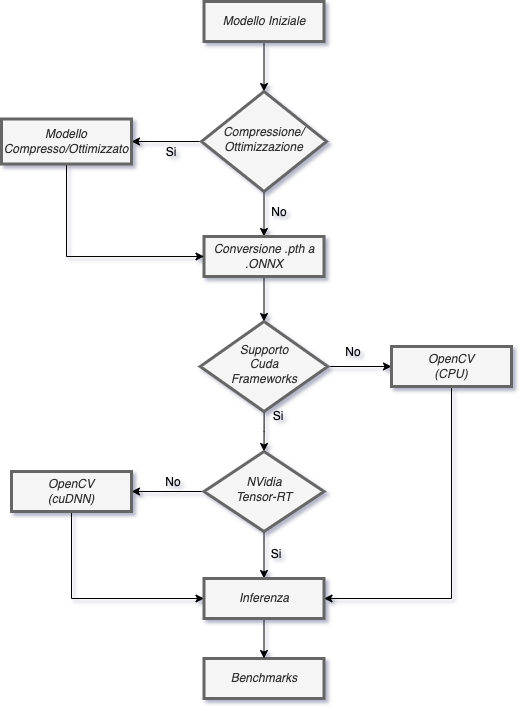
\includegraphics[width = \linewidth]{flow_chart.png}
    \centering
    \caption{Flusso di esecuzione di ogni modello.}
    \label{flow_chart}
\end{figure}

\section{NVidia Jetson Nano}
La Jetson Nano (B01), presentata nel Marzo del 2019,  è una scheda embedded 
sviluppata da NVidia che rappresenta il prodotto più piccolo della 
famiglia Jetson. L'utilizzo della scheda è rivolto principalmente verso varie 
applicazioni di intelligenza artificiale, visione artificiale e robotica. A bordo 
troviamo un processore e una scheda madre che offre una potenza di calcolo 
pari a 128 Cuda cores. L'obiettivo di questa scheda è quello di funzionare 
con reti neurali e offrire le migliori prestazioni quando viene utilizzata per 
eseguire inferenze. A differenza di altre architetture, lo Jetson Nano utilizza 
una precisione Floating point (FP) a 16-bit che lo rende competitivo rispetto 
ad altri device embedded. Purtroppo non supporta la precisione a 8-bit 
ma è comunque in grado di lavorare con qualsiasi rete disponibile e con 
qualsiasi framework di deep learning popolare (es: Pytorch, TensorFlow, 
Keras, Caffe etc.). In questo dispositivo è possibile effettuare sia il rilascio 
(deploy) dell'applicazione che l'addestramento della rete ma, in quest'ultimo 
caso, risulta essere lento a causa delle prestazioni computazionali ridotte. 
Risulta inoltre possibile effetuare operazioni di transfer learning tra i modelli.
Oltre ad avere il vantaggio delle dimensioni ridotte, un altro principale vantaggio 
della Jetson Nano deriva dall'applicazione dell'acceleratore TensorRT. 
Quest'ultimo esegue un processo di quantizzazione che è utile a convertire i 
pesi e gli input in precisioni Floating Point inferiori, in modo da preservare 
la memoria che, su una scheda del genere, rappresenta una limitazione. A 
tal proposito, il dispositivo non fornisce alcun tipo di memoria integrata, 
ma esiste la possibilità di aggiungerne una grazie alla presenza di uno slot 
di espansione in cui è possibile alloggiare una scheda micro-sd. Essendo una 
scheda embedded, a differenza di altri computer che utilizzano alimentatori 
da diversi Watts (W), la Jetson Nano può utilizzare due diversi livelli di 
wattaggio. Il primo, quello da 5W, raggiungibile grazie alla presenza di 
una porta micro-usb, mentre il secondo, quello da 10W, è raggiungibile solo 
grazie all'utilizzo di un alimentatore esterno collegato tramite l'ingresso 
jack. Il massimo livello di performance, raggiungibile dalla GPU, avviene 
proprio tramite l'utilizzo dell'alimentatore esterno. Per rendere l'idea delle 
dimensioni e dell'intera architettura, in Figura (\ref{jetson}) è riportata la Jetson 
Nano.
\begin{figure}[]
    \begin{minipage}[t]{.45\textwidth}
        \centering
        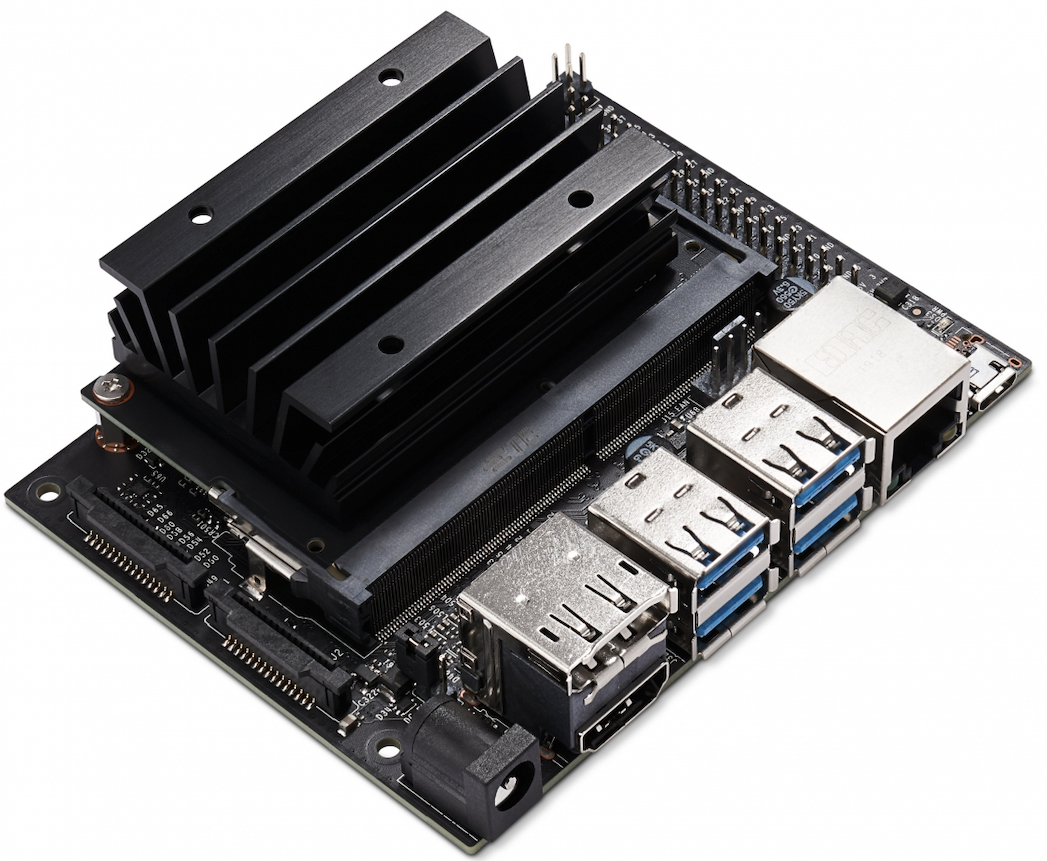
\includegraphics[width=\textwidth]{jetson1.png}
    \end{minipage}
    \hfill
    \begin{minipage}[t]{.45\textwidth}
        \centering
        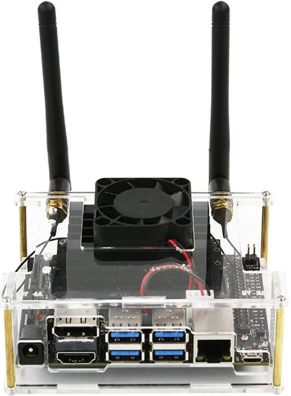
\includegraphics[width= 0.8\textwidth]{jetson2.png}
    \end{minipage}  
    \caption{NVidia Jetson Nano.}
    \label{jetson}
\end{figure}

\section{Modelli}
Il lavoro di tesi è incentrato nello studio di diversi modelli profondi e nell'applicazione, del tutto personalizzata, di una nota tecnica di compressione/ottimizzazione su uno di questi. Lo scopo è quello di aumentare la velocità di inferenza, nonché i Frames-Per-Second (FPS), in modo da permettere la sua implementazione su diverse architetture anche con limitate risorse computazionali (es: Jetson Nano). Per arrivare all'obiettivo finale, si è partito dallo studio delle performance ottenute da diversi modelli pre-addestrati messi a disposizione dalla community di NVidia. Dopo aver ottenuto i risultati, lo studio si è incentrato sull'utilizzo di una particolare architettura di rete, nota con il nome di \emph{MobileNet-V1}, con l'obiettivo di migliorarla. Successivamente il focus si è spostato nell'implementazione di tale rete in una seconda architettura, quest'ultima avente il nome di \emph{Single-Shot-Detector (SSD)}. Prima di giungere ai risultati ottenuti, è fondamentale avere un'ampia visione dei modelli utilizzati e di come questi hanno evidenziato le capacità computazionali delle architetture utilizzate. 
\subsection{Modelli pre-addestrati}
I modelli messi a disposizione da NVidia hanno permesso da subito di estrarre le vere potenzialità di tutte le architetture di studio. Grazie alla presenza di uno script eseguibile nelle librerie jetson utils (ref Jetson utils), sono stati reperiti diversi modelli, allenati su diverse tipologie di datasets, divisi in due categorie: Object Detection (Tab. \ref{pre_trained_models_obj_det}) e Semantic Segmentation (Tab. \ref{pre_trained_models_sem_seg}).
Tutti i modelli riportati sono stati testati su tutte le architetture di riferimento. Nuovamente si ricorda al lettore che lo scopo della tesi è aumentare codeste performance. Il produttore ha eseguito alcuni test sulla velocità di inferenza solamente su alcuni dei modelli proposti. Per poter visualizzare i risultati ottenuti, si rimanda la lettura al capitolo successivo.
\begin{table}[]
    \renewcommand{\baselinestretch}{1}
    \centering
    \begin{adjustbox}{max width=\textwidth}
    \begin{tabular}{|c||L|L||}
        \hline
        \multirow{2}{*}{\bfseries{MODELLI}} & \multicolumn{2}{c||}{\bfseries{OBJECT DETECTION}}\\            & \bfseries{Dataset} & \bfseries{Risoluzione}\\
        \hline
        \hline
        {\bfseries{SSD-MOBILENET-V1}} & MS COCO & 640$\times$480\\
        \hline
        {\bfseries{SSD-MOBILENET-V2}} & MS COCO & 640$\times$480\\
        \hline 
        {\bfseries{SSD-INCEPTION-V2}} & MS COCO & 640$\times$480\\
        \hline
        {\bfseries{PEDNET}} & MS COCO & 640$\times$480\\
        \hline
        {\bfseries{MULTIPEDNET}} & MS COCO & 640$\times$480\\
        \hline
    \end{tabular}
    \end{adjustbox}
    \vspace{0.5cm}
    \caption{Modelli pre-addestrati utilizzati per l'attività di object detection.}
    \label{pre_trained_models_obj_det}
\end{table}

\begin{table}[]
    \renewcommand{\baselinestretch}{1}
    \centering
    \begin{adjustbox}{max width=\textwidth}
    \begin{tabular}{|c||L|L||}
        \hline
        \multirow{2}{*}{\bfseries{MODELLI}} & \multicolumn{2}{c||}{\bfseries{SEMANTIC SEGMENTATION}}\\            & \bfseries{Dataset} & \bfseries{Risoluzione}\\
        \hline
        \hline
        {\bfseries{FCN-RESNET-18}} & Cityscapes & 512$\times$256\\
        \hline
        {\bfseries{FCN-RESNET-18}} & Cityscapes & 1024$\times$512\\
        \hline 
        {\bfseries{FCN-RESNET-18}} & Cityscapes & 2048$\times$1024\\
        \hline
        {\bfseries{FCN-RESNET-18}} & Pascal Voc & 320$\times$320\\
        \hline
        {\bfseries{FCN-RESNET-18}} & Pascal Voc & 512$\times$320\\
        \hline
    \end{tabular}
    \end{adjustbox}
    \vspace{0.5cm}
    \caption{Modelli pre-addestrati utilizzati per l'attività di semantic segmentation.}
    \label{pre_trained_models_sem_seg}
\end{table}

\subsection{Modello base di riferimento}\label{MBNET}
Per verificare la veridicità dei risultati ottenuti e quelli dichiarati dal produttore, l'intero lavoro di tesi si è concentrato maggiormente nella ricerca e nella costruzione di un modello "from scratch". Per aver un confronto equo, dopo diversi studi focalizzati sulle varie architetture dei modelli pre-addestrati, la scelta è ricaduta sull'implementazione della rete \emph{MobileNet-V1}. Questa decisione è motivata nelle sezioni più avanti quando si discuterà delle tecniche di compressione/ottimizzazione adottate. 
Approfondendo il paper scientifico \cite{howard2017mobilenets}, o scopo degli autori è quello di creare un'architettura di rete dinamica, influenzata dalla presenza di diversi iper-parametri, adattabile in diversi dispositivi compresi quelli mobili. L'architettura della rete MobileNet-V1 è raffigurata in Figura \ref{mobilenetV1}:
\begin{figure}
    \centering
    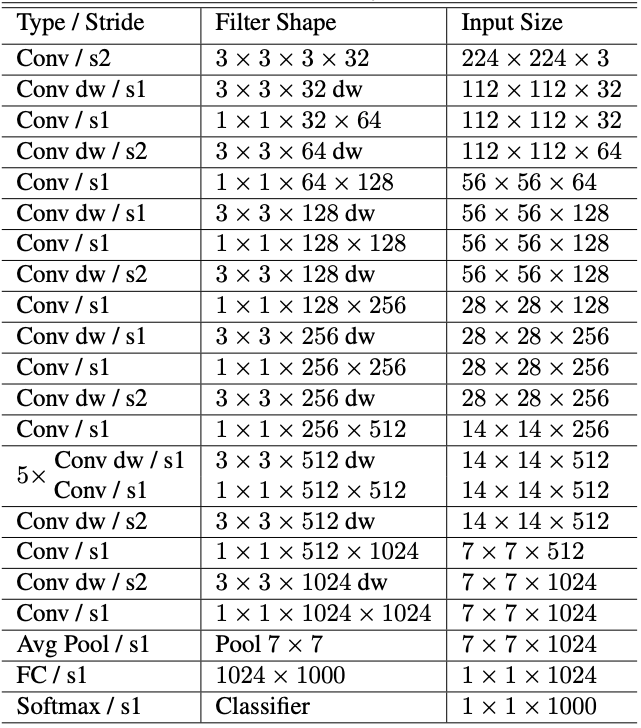
\includegraphics[width = 0.9\linewidth]{mobilenet_architecture.png}
    \centering
    \caption{Architettura MobileNet-V1.}
    \label{mobilenetV1}
\end{figure}
La particolarità che contraddistingue la seguente rete dalle altre è basata sulla presenza di convoluzioni personalizzate chiamate "\emph{Depthwise Separable Convolutions}"  che, a differenza delle comuni convoluzioni, fattorizzano una convoluzione standard prima in una convoluzione profonda e successivamente in una convoluzione 1x1 chiamata "pointwise convolution", formando due layers distinti (Fig. \ref{depth_wise}).
\begin{figure}
    \centering
    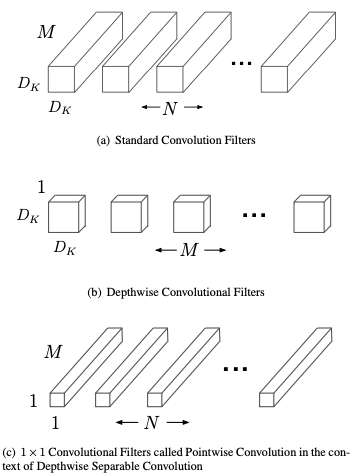
\includegraphics[width = 0.8\linewidth]{depth_wise.png}
    \centering
    \caption{La convoluzione standard (a) viene sostituita da due layers: depthwise convolution (b) e pointwise convolution (c) per costruire un depthwise separable filter.}
    \label{depth_wise}
\end{figure}
La prima convoluzione ha l'obiettivo di applicare un singolo filtro per ogni canale in input, mentre la seconda creare una combinazione lineare dell'output. Lo scopo della fattorizzazione è quello di ridurre drasticamente la computazione e le dimensioni del modello. Tutti i livelli sono seguiti da una normalizzazione batch e una funzione di attivazione ReLU, ad eccezione del livello finale che è un completamente connesso. Il tutto termina con una Softmax utile per la classificazione. In totale, MobileNet ha 28 livelli le costituiscono la profondità dell'intera rete. Per costruire una rete a dimensioni ridotte, con un numero di parametri inferiore, beneficiando di un incremento di velocità, gli autori hanno introdotto due tipologie di parametri, uno dei quali risultate molto importanti per raggiungere l'obiettivo di questa tesi. I  due parametri prendono il nome di: 
\begin{enumerate}
    \item \emph{Width Multiplier ($\alpha$)}
    \item \emph{Resolution Multiplier ($p$)}
\end{enumerate}
Il ruolo del width multiplier $\alpha$, un valore tra 0 e 1 compreso, è quello di ridurre le dimensioni della rete in modo uniforme su ogni strato. Per quanto riguarda l'iper-parametro Resolution multiplier $p$,  il suo scopo è quello di accelerare l'inferenza della rete andando ad agire sull'immagine in input e nella rappresentazione interna di ogni livello. In poche parole, l'intento di quest'ultimo parametro è quello di ridurre la  risoluzione dell'immagine di input, e delle successive sue elaborazioni, per poter incrementare la velocità. Il decremento portato da questo parametro fa sì che la risoluzione possa raggiungere uno dei seguenti valori $p=\{224, 192, 160, 128\}$.
Nel complesso, l'utilizzo di questa architettura ha permesso la composizione dell'architettura di rete \emph{Single-Shot-Detector (SSD)}. 

\subsection{Modello Single Shot Detector}
Nella sezione precedente sono state riportate tutte le caratteristiche che contraddistinguono una rete MobileNet-V1 rispetto alla concorrenza. Tale rete risulta sostanziale per formare l'ultima architettura di rete che sarà utilizzata per ricavare i risultati attesi. Il nuovo modello di rete prende il nome di \emph{Single-Shot-Detector (SSD)}.
Una SSD è una rete convoluzionale feed-forward in grado di produrre dei riquadri di delimitazione (bounding-boxes o anchor-boxes), di dimensione fissa, con i relativi punteggi associati alle istanze di ogni classe presenti in ognuno dei riquadri. L'ultima operazione applicata, che in gergo viene chiamata "Non-Maximum Suppression" (NMS), è utile per selezionare il riquadro migliore tra tutti quelli prodotti su ogni specifico oggetto. 
L'architettura una SSD contiene nei primi livelli una "rete base" (backbone), avente il livello di classificazione finale (FC) rimosso, utilizzata per la classificazione delle immagini. Oltre a questa sezione, una SSD si contraddistingue in merito all'aggiunta di ulteriori livelli a seguire, aventi lo scopo di:
\begin{itemize}
    \item \emph{Produrre feature-maps multi-scala}: l'idea è quella di produrre previsioni su identificazioni in più scale. Ogni strato convoluzionale aggiunto produrrà una feature map sulla quale si potranno identificare gli oggetti in scale diverse. Le dimensioni di questi livelli diminuiranno all'aumentare della profondità della rete;
    \item \emph{Generare delle predizioni}: grazie all'inserimento degli ulteriori livelli, si ha la possibilità di produrre un set di predizioni sulle identificazioni tramite l'utilizzo di un insieme di filtri. Con l'applicazione di un filtro convoluzionale di dimensioni $3x3xp$, dove p sta ad indicare i canali, su ogni cella, l'intero modello riesce a produrre un punteggio per ogni categoria, con tanto di coordinate correlate alla regione di delimitazione. Ogni filtro produrrà un numero di punteggi pari al numero di classi (background compreso). Per esempio, in Conv4\_3 (Fig. \ref{SSD_Arch}), viene applicato un filtro 3x3 utile a mappare 512 canali di input in 25 canali di output. Le coordinate prodotte, verranno confrontate rispetto a determinate anchor-boxes associate a diverse posizioni in ogni feature map;
    \item \emph{Generare dei riquadri di delimitazione}: normalmente vengono associati dei riquadri standard (anchor box) ad ogni feature map risultante dai livelli convoluzionali aggiunti. Il calcolo di un offset permette di generare delle nuove bounding boxes che meglio si adattano all'oggetto nell'immagine. 
\end{itemize}
Invece di utilizzare altri metodi, come la finestra scorrevole (sliding windows), per determinare la posizione di ogni oggetto viene sovrapposta una griglia dove, all'interno di ogni cella, è possibile identificare la presenza di un oggetto. Se non vi ci fosse alcun oggetto all'interno di una regione, allora tale cella sarà classificata come "background" e la posizione verrà ignorata. A volte, all'interno di ogni cella, ci possono essere molteplici oggetti, appartenenti a diverse categorie, in forme diverse. Per poterli rilevare, bisogna introdurre i concetti di "\emph{anchor box}" e di "\emph{receptive field}". 
Un anchor-box è un riquadro, di dimensioni predefinite, responsabile della dimensione e della forma di un oggetto all'interno di una cella che a sua volta può avere più di una anchor-box. Durante l'allenamento di una SSD, viene eseguita una fase di corrispondenza tra il miglior l'anchor-box e il riquadro di delimitazione presente nel ground-truth delimitante uno specifico oggetto. Dopo aver trovato l'anchor-box con il più alto grado di sovrapposizione ad un oggetto, si può procedere alla predizione della classe e alla localizzazione della sua posizione. Ogni anchor-box e determinato sia da un valore di aspect-ratio che da un livello di zoom. L'aspect-ratio determina la forma di una anchor-box in base all'oggetto sottostante. Il parametro zoom invece, è utile per specificare la quantità di ridimensionamento di ogni anchor-box rispetto a ciascuna cella.
In ogni feature map, per ogni anchor-box verranno calcolati i punteggi di tutte le classi c e 4 offset complessivi relativi alla forma dell'anchor-box nel ground-truth, per un numero totale di output pari a:
\begin{equation}
    (c+4)kmn
\end{equation}
dove:
\begin{itemize}
    \item $c$: numero di classi (compresa la classe background);
    \item $4$: numero di offsets per ogni anchor-box;
    \item $k$: numero di anchor-boxes per ogni posizione;
    \item $m \times n$: dimensione feature map;
    \item $(c+4)k$: numero di filtri applicati ad ogni posizione della feature map.
\end{itemize}
Prendendo sempre in riferimento la Figura \ref{SSD_Arch}, sulla convoluzione 4\_3 di dimensioni $38x38x512$, viene applicato un filtro, di dimensioni $3x3$.
Successivamente verranno calcolate le 4 anchor-boxes che, in maniera individuale, produrranno un numero di output pari a $(c+4)$. Pertanto, tale livello convoluzionale produrrà un output di $38x38x4x(c+4)$.
In termini di numero di anchor-boxes, saranno prodotti $38x38x4=5776$ riquadri. Proseguendo con il calcolo, il numero totale di riquadri generati è per ogni classe è pari a 8732.
La creazione di multiple predizioni sotto forma di riquadri e di punteggi, è chiamata multibox. 

\begin{figure}
    \centering
    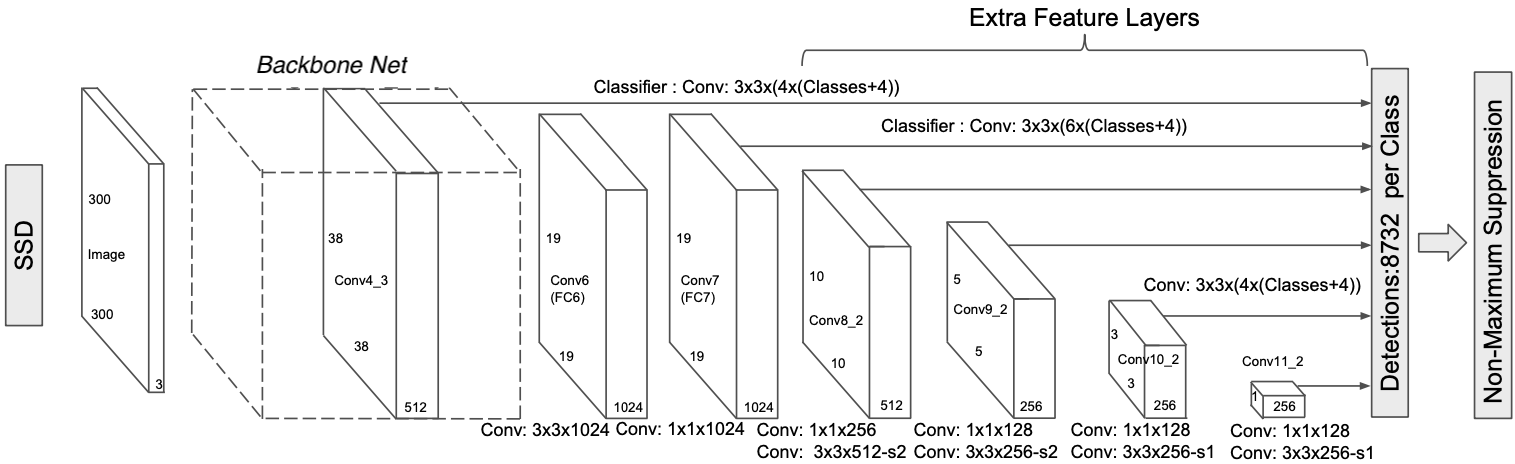
\includegraphics[width =\linewidth]{SSD_architecture.png}
    \centering
    \caption{Architettura Single-Shot-Detector (SSD).}
    \label{SSD_Arch}
\end{figure}

\subsection{Modello Distilled-Single-Shot-Detector (DSSD)}
Dopo aver elencato, nelle sezioni precedenti, i diversi modelli utilizzati, in questa sezione verrà definito il modello finale proposto su cui si concentreranno tutti gli sforzi del seguente elaborato. Come già accennato, il focus del sottoscritto si è incentrato principalmente verso l'utilizzo di due architetture di rete utili a compire l'attività di object detection. Il modello finale si basa nell'implementazione della rete MobileNet-V1 come rete base nell'architettura Single-Shot-Detector. L'unione tra queste due architetture crea un unico modello nominato \emph{SSD-MobileNet-V1}.
Il numero di livelli presenti in ogni parte della rete sono:
\begin{itemize}
    \item \emph{27 livelli} (di default sono 28 escludendo l'AvgPool e il Softmax) rappresentanti la rete base (backbone) da cui è stato rimosso il livello FC;
    \item \emph{8 livelli convoluzionali extra}, seguiti da 8 funzioni di attivazione ReLU.
    \item \emph{6 livelli convoluzionali} utilizzati per la \emph{regressione};
    \item \emph{6 livelli convoluzionali} utilizzati per la \emph{classificazione};
\end{itemize}
Dopo aver inserito la nuova rete base, colleghiamo i livelli depth-wise 12 e 14 alla restante parte della rete SSD. Entrambi i livelli hanno filtri di dimensione pari a $1x1x512x512$ , che a loro volta producono due feature maps aventi profondità 512. L'ultimo collegamento effettuato riguarda l'ultimo livello di convoluzione "pointwise" avente dimensioni $1x1x1024x1024$.
La scelta di questi livelli è attribuita al loro contenuto informativo. In quella determinata posizione, i layers contengono sia features di alto livello che di basso livello. Dal punto di vista pratico, le predizioni vengono eseguite utilizzando i livelli di classificazione e regressione. Per ogni output prodotto dalla rete base, ci sono differenti livelli collegati (Fig. \ref{SSD_conn}) aventi lo scopo di rilevare gli oggetti aventi diverse dimensioni e proporzioni. Tali livelli sono formati da piccoli kernel $3x3$ con uno passo (stride) uguale a 1 e funzionano nel seguente modo:
\begin{itemize}
    \item Ogni layer di classificazione viene associato ad una particolare anchor-box esistente e all'aspect-ratio di un particolare output della rete. Codesto, durante l'addestramento, impara a rilevare una particolare classe di oggetti;
    \item Ogni layer di regressione è anch'esso associato a una anchor-box e al suo aspect-ratio. Durante l'allenamento questi apprendono come definire un offset per una determinata anchor-box che è parzialmente contenuta in una anchor-box predefinita. Questa componente pertanto è responsabile di produrre i riquadri di delimitazione.
\end{itemize}
Nelle prossime sezioni verranno elencate tutte le operazioni riguardanti le modifiche apportate a codesta architettura che hanno permesso di ottenere i risultati sperati.
\begin{figure}
    \centering
    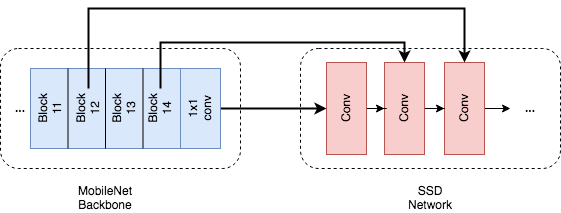
\includegraphics[width =\linewidth]{connection_SSD.png}
    \centering
    \caption{Connessioni tra i livelli della rete base (MobileNet) e i livelli della rete SSD.}
    \label{SSD_conn}
\end{figure}

\section{Compressione/Ottimizzazione del modello proposto}
Avendo definito l'architettura del modello proposto, nella seguente sezione vengono descritti tutti i suoi impieghi in alcune delle tecniche di compressione/ottimizzazione descritte nel capitolo due. L'affermazione "alcune"sta ad indicare l'esclusione della tecnica di quantizzazione in quanto la minima precisione supportata dalla scheda embedded Jetson Nano è la FP16 (default). Non potendo applicare la precisione INT8 su quest'ultima, lo studio ha tralasciato l'implementazione pratica di tale tecnica soffermandosi solo a livello teorico. Le altre due tecniche invece, sono state ampiamente utilizzate per condurre dei test sul modello proposto. Di seguito verranno mostrati tutti i procedimenti, eseguiti con entrambe le tecniche, utili a ricavare i risultati finali.

\subsection{Pruning sul modello proposto}\label{pruning_model}
Riprendendo il concetto cardine su cui è focalizzata la tecnica di Pruning\index{Pruning}, è stato possibile svilupparne una sua implementazione con l'aiuto del noto framework di machine learning: PyTorch. Sfortunatamente, la tecnica di pruning\index{Pruning} messa a disposizione da codesto (ancora in fase beta) non migliora i tempi di inferenza del modello proposto. Questa causa è da attribuirsi alla non riduzione delle dimensioni dovuta dall'utilizzo di tensori densi all'interno del modello. Un tensore del genere, se riempito di zeri, non esegue calcoli veloci ed inoltre non occupa una dimensione ridotta quando viene memorizzato sul disco. Questa rappresenta una limitazione da parte di questa tipologia di tensori. Di conseguenza, il team di PyTorch afferma che lo scopo, della tecnica messa disposizione, non è incentrato nel garantire incrementi di velocità o risparmi di memoria ma rappresenta un concetto sperimentale. Giusto per non penalizzare solamente PyTorch, anche TensorFlow presenta questa limitazione, ma entrambi hanno intenzione di proseguire lo sviluppo di tale tecnica introducendo nuove migliorie. Attualmente, l'unico fattore da cui si può trarre un vantaggio, riguarda l'applicazione dei programmi di compressione, come per esempio gzip, sui modelli sottoposti al \index{Pruning}. 
Per quanto riguarda il lato implementativo, si è deciso di applicare la tecnica sul modello SSD-MobileNet-V1 precedentemente definito. Come si è potuto notare nel sottoparagrafo apposito, la struttura del modello è composta da diversi livelli quali convoluzionali (Conv2D), Normalizzazione Batch (BatchNorm2D), ReLU (per l'attivazione) e Fully Connected (per l'output). Dovendo azzerare i parametri più numerosi, ci si concentrerà maggiormente sui pesi, a loro volta presenti in quantità maggiore nei livelli convoluzionali. 
La tecnica di pruning\index{Pruning} utilizzata è la one-shot.
La funzioni di pruning\index{Pruning} messe a disposizione di PyTorch sono racchiuse nel modulo torch.nn.utils.prune. Grazie alla presenza di un parametro, chiamato "sparsity" (sparsità), si può indicare la percentuale di parametri da azzerare. Le tecniche utilizzate sono le seguenti:
\begin{itemize}
    \item \emph{Unstructured (Non-strutturata)}: reperibile in \emph{torch.nn.prune.l1\_unstructured}. La tecnica applica la potatura in base al magnitudo di ogni peso (norma L1), in maniera individuale in ogni livello. Questa rappresenta la forma più semplice di potatura di un modello;
    \item \emph{Structured (Strutturata)}:  utilizzabile con \emph{torch.nn.prune.ln\_structured}. Questa tecnica incide direttamente sui canali di output andando a rimuovere la porzione di filtri con il punteggio più basso nel livello convoluzionale. La seguente tecnica risulta essere meno fedele rispetto a quella non strutturata;
    \item \emph{Global Unstructured (Globalmente Non-strutturata)}: richiamabile tramite \emph{torch.nn.prune.global\_unstructured}, rappresenta la tecnica che ci fornisce un riscontro globale sulla quantità di pesi da poter rimuovere nell'intero modello.
\end{itemize}
L'API permettono facilmente di utilizzare il modello sia con i parametri originali oppure direttamente con i parametri potati preservando in quest'ultimo caso la struttura originale. Semplicemente, i tensori originali vengono salvati sotto il nome di "\emph{weigth\_orig}", mentre quelli potati vengono salvati in un apposito buffer, chiamato "\emph{weigth\_mask}", contenente tutte le maschere nulle. L'applicazione delle maschere di zeri avviene mediante l'utilizzo di un \emph{forward hook}. Giusto per riportare una breve descrizione, un forward hook è una funzione che viene eseguita quando viene chiamato il metodo "forward" o "backward". Lasciando entrambi i seti di pesi, le dimensioni del modello aumenteranno quando questo verrà salvato su disco. Non essendo lo scopo finale, si procederà ad eliminare i pesi originali rendendo permanenti quelli presenti nella maschera. Per fare ciò è possibile richiamare il metodo \emph{prune.remove}. 
Per quanto riguarda lo spazio occupato in memoria, le tecniche di potatura sembrano avere una relazione lineare con la dimensione di un modello compresso. Questo fenomeno accade a causa della serializzazione effettuata dagli algoritmi di compressione.
Questo benefit è molto richiesto, sia in fase di rilascio che di inferenza, su un dispositivo con bassa disponibilità su disco. Ovviamente, maggiore sarà l'indice di sparsità e maggiore sarà lo spazio recuperato. 

\subsection{Knowledge Distillation sul modello proposto}\index{Knowledge Distillation}\label{KD_steps}
Terminata l'analisi sulle possibili applicazioni della tecnica di Pruning\index{Pruning}, e a quali vantaggi e svantaggi può portare, in questa sezione saranno analizzati tutti gli aspetti derivanti dall'implementazione della seconda tecnica di compressione/ottimizzazione. Il modello finale, derivante dall'applicazione della tecnica di Knowledge distillation\index{Knowledge Distillation}, è stato ricavato tramite l'esecuzione dei sei seguenti passaggi mostrati in Figura \ref{steps_KD}.
\begin{figure}
    \centering
    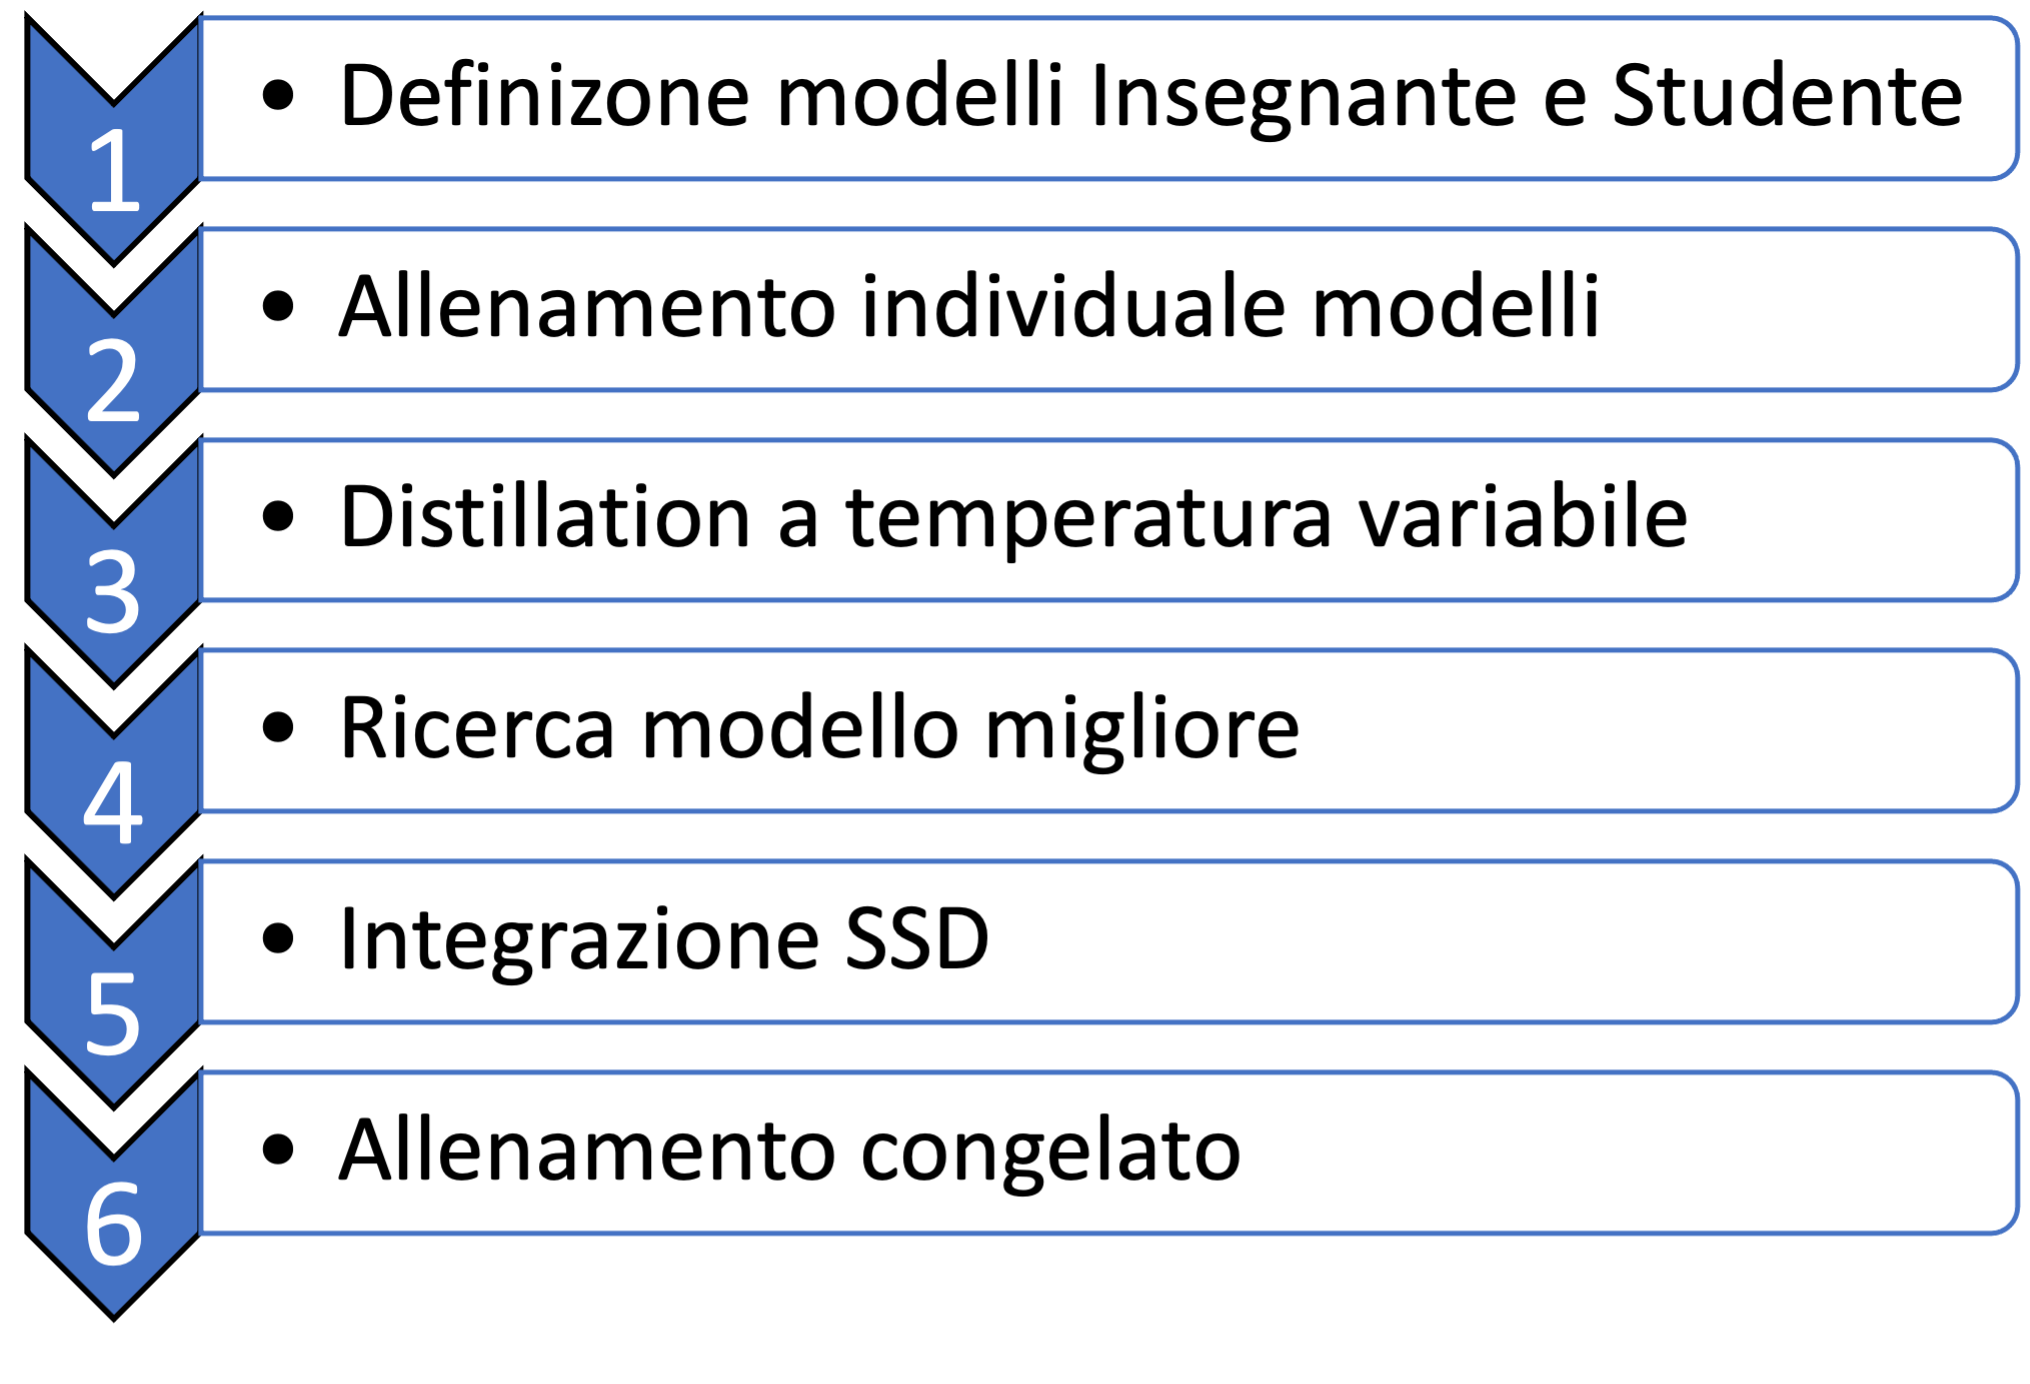
\includegraphics[width =\linewidth]{steps_KD.png}
    \centering
    \caption{Steps per la produzione del modello distillato finale.}
    \label{steps_KD}
\end{figure}

\subsubsection{1. Definzione modelli Insegnante e Studente}
Per la generazione del modello distillato, occorre possedere un modello Insegnante in grado di poter trasmettere la propria conoscenza verso un altro modello. Il modello insegnante utilizzato è il modello base di riferimento (Sezione \ref{MBNET}) MobileNet-V1. Prendendo in riferimento la sua architettura, affinché possa essere applicato il concetto di Knowledge distillation\index{Knowledge Distillation}, che si basa nel trasferire la conoscenza da un modello di grande dimensioni verso un modello di piccole dimensioni, bisogna creare un secondo modello chiamato Studente. Secondo la letteratura, l'architettura dello studente dovrà essere simile, in termini di profondità, a quella dell'insegnante. Per soddisfare il seguente vincolo,  ci viene in aiuto l'iper-parametro "width multiplier" ($\alpha$), ideato direttamente dagli autori della rete di riferimento. L'integrazione di tale permette di non incidere sulla profondità della rete ma bensì sul suo numero di parametri, raggiungendo un costo computazionale pari a:
\begin{equation}
    D_K \cdot D_K \cdot \alpha M \cdot D_F \cdot D_F + \alpha M \cdot \alpha N \cdot D_F \cdot D_F
\end{equation}
dove:
\begin{itemize}
    \item $D_K$: Dimensioni spaziali del kernel in una convoluzione;
    \item $D_F$: Dimensioni spaziali feature map;
    \item $M$: numero di canali in input;
    \item $N$: numero di canali in output;
    \item $\alpha$: width multiplier compreso tra 0 e 1 incluso.
\end{itemize}
Il valore del parametro $\alpha$ utilizzato è pari a 0.25. Moltiplicando tale valore al numero di canali di input e di output, si ottiene un modello più piccolo, di un fattore pari a $1/4$, rispetto al modello insegnante concepito con un valore standard $\alpha=1$. Per facilitare i prossimi calcoli, non è stato ritenuto opportuno implementare anche l'iper-parametro "resolution multiplier" (\emph{p}) in quanto interferente con le diverse dimensioni delle feature maps generate nel comparto SSD. Tralasciando questo elemento, gli autori di MobileNet-V1 affermano che un modello ricavato da tale parametro, oltre ad avere delle dimensioni ridotte e un costo computazionale minore, ha un livello di accuratezza leggermente minore rispetto al modello più grande (insegnante). 

\subsubsection{2. Allenamento individuale modelli}
Giunti a questo punto, i modelli a disposizione sono due; un modello Insegnante e un modello Studente. Per poter eseguire gli steps successivi, occorre allenare entrambi i modello per poter ricavare le loro accuratezze utili in seguito. Pertanto, si il seguente step si basa nell'allenare entrambi i modelli sulle immagini fornite dal dataset "\emph{Open Images}". Le categorie utilizzate, rappresentanti le etichette (labels), essendo in un contesto di guida autonoma, sono le seguenti: Bicicletta, Bus, Auto, Motociclo, Persona, Semaforo, Cartello stradale e Camion. Ogni modello verrà addestrato per un numero totale di 1000 epoche sull'intero set di allenamento (training set). Il reperimento delle immagini è avvenuto grazie a uno script in grado di creare tre diversi insiemi: allenamento, test e valutazione. In totale, il numero di immagini suddiviso per ogni categoria è riportato nella Tabella \ref{images_train}.
\begin{table}
    \centering
    \begin{adjustbox}{max width=\textwidth}
    \begin{tabular}{|c|c|}
        \hline
        \bfseries{Categorie} & \bfseries{\#Immagini}\\
        \hline
        \hline
        Biciclette & 536 \\
        \hline
        Bus & 157 \\
        \hline
        Auto & 3616 \\
        \hline
        Motocicli & 206\\
        \hline
        Persone & 12094\\
        \hline
        Semafori & 102\\
        \hline
        Segnali stradali & 63\\
        \hline
        Camion & 159\\
        \hline
        \hline
        {\bfseries{Totale}} & {\bfseries{16933}} \\
        \hline
    \end{tabular}
    \end{adjustbox}
    \vspace{0.5cm}
    \caption{Numero di immagini per ogni cateogria.}
    \label{images_train}
\end{table}
La somma del numero delle immagini costituisce un insieme di 16933 elementi, tutti suddivisi nei tre insiemi. Tutti gli allenamenti sono stati eseguiti esclusivamente sull'architettura Google Colaboratory Pro per una ragione legata prettamente alla velocità temporale messa a disposizione da un hardware costruito ad hoc. Oltre al parametro $\alpha$, gli iper-parametri utilizzati durante l'allenamento riguardano: batch size = 8, learning rate = 0.1, momento = 0.9 e weigth decay = 1e-4. Per quanto riguarda la risoluzione delle immagini in input, queste venivano ridimensionate a una risoluzione pari a 224x224. Per quanto riguarda i tempi di allenamento, sempre su 1000 epoche, il modello insegnante ha impiegato circa 11 ore per concludere contro le 9 ore impiegate dal modello studente. La riduzione dei tempi di allenamento è dovuta alle ridotte dimensioni del modello studente rispetto al modello insegnante. 

\subsubsection{3. Distillation a temperatura variabile}
Fino a questo punto sono stati elencati gli elementi fondamentali su cui creare una base di partenza. Avendo a disposizione i due principali modelli, si procede con la vera e propria applicazione della tecnica di Knowledge distillation\index{Knowledge Distillation}. Prendendo sempre in riferimento tutti i concetti riportati nella sezione \ref{KD_distill} del capitolo 2, l'elemento ritenuto parte integrante di tale tecnica è la temperatura T. Lo scopo è quello avvalersi delle soft-targets per realizzare diversi modelli di studenti a diverse temperature, integrando il trasferimento della conoscenza distillata. 
Si ricorda che la nozione di temperatura è prettamente legata ad un concetto di generalizzazione. La lista di temperature utilizzate è: $T=\{1, 2, 3, 4, 5, 10, 15\}$.
Ogni modello generato deriva anch'esso da un allenamento, ognuno di circa 9 ore, su 1000 epoche, in cui sono stati sottoposti gli stessi insiemi di immagini (batch), sia al modello insegnante che al modello studente base. Il passaggio dell'intero training set ad entrambi i modelli ha permesso di migliorare la perdita generale, che ricordo essere la somma delle perdite dei due modelli. Gli iper-parametri, così come l'intero set di immagini, utilizzati per l'allenamento sono gli stessi utilizzati per allenare i modelli base. Ricapitolando, ciò che si vuole ottenere da questo passaggio riguarda la generazione di multipli modelli di studenti su cui si baseranno i prossimi steps. 

\subsubsection{4. Ricerca modello migliore}
Dopo aver generato i sette nuovi modelli distillati, bisogna chiedersi quale tra questi scegliere. Per ottenere una risposta, bisogna ricavare i tassi di errori (\emph{Errors rates}) sul set di validazione prodotto da ognuno di loro o, in altri termini, bisogna ricavare la curva di apprendimento di ogni modello. Tale curva mette in risalto gli errori effettuati in fase di validazione in ogni epoca. Il valori minimi e massimi sono gli errori presi in considerazione e sono visibili nella Tabella \ref{error_rates_T}.
\begin{table}
    \renewcommand{\baselinestretch}{1}
    \centering
    \begin{adjustbox}{max width=\textwidth}
    \begin{tabular}{|c||L|L||L|L|}
        \hline
        \multirow{2}{*}{\bfseries{MODELLI}} & \multicolumn{2}{c||}{\bfseries{IPER-PARAMETRI}} & \multicolumn{2}{c|}{\bfseries{ERRORI}}\\  & \bfseries{$\alpha$} & \bfseries{T}  & \bfseries{Min} & \bfseries{Max} \\
        \hline
        \hline
        {\bfseries{Insegnante}} & / & / & \color{blue}{\bfseries{32}} & \color{blue}{\bfseries{76}}\\
        \hline
        {\bfseries{Studente base}} & 0.25 & / & \color{blue}{\bfseries{40}} & \color{blue}{\bfseries{73}}\\
        \hline 
        {\bfseries{Studente-Dst}} & 0.25 & 1 & \color{red}36 & \color{red}74\\
        \hline
        {\bfseries{Studente-Dst}} & 0.25 & 2 & \color{red}43 & \color{red}76\\
        \hline
        {\bfseries{Studente-Dst}} & 0.25 & 3 & \color{green}{\bfseries{38}} & \color{green}{\bfseries{76}}\\
        \hline
        {\bfseries{Studente-Dst}} & 0.25 & 4 & \color{red}49 & \color{red}73\\
        \hline
        {\bfseries{Studente-Dst}} & 0.25 & 5 & \color{red}41 & \color{red}73\\
        \hline
        {\bfseries{Studente-Dst}} & 0.25 & 10 & \color{red}50 & \color{red}76\\
        \hline
        {\bfseries{Studente-Dst}} & 0.25 & 15 & \color{red}53 & \color{red}77\\
        \hline
    \end{tabular}
    \end{adjustbox}
    \vspace{0.5cm}
    \caption{Errors Rates dei modelli Insengante, Studente base e Studente distillato (Dst) a diverse temperature T. I valori in blu sono quelli di riferimento, mentre quelli verdi rappresentano gli errori derivanti dal modello scelto.}
    \label{error_rates_T}
\end{table}
Per la scelta del modello migliore, affinché venga soddisfatto il principio di generalizzazione, un primo vincolo ci impone di scegliere un modello ricavato da una temperatura maggiore di uno. La scelta quindi si restringe ad un range di modelli i cui errori, minimo e massimo, fossero compresi tra gli indici di errore del modello insegnante e del modello studente base. Sempre in riferimento alla Tabella \ref{error_rates_T}, il valore di errore minimo deve essere compreso tra io valori 32 e 40 (incluso), mentre il valore massimo deve essere minore o uguale di 76. Il primo modello che rispetta tali condizioni è quello ricavato da una temperatura T=3. Per verificare la giusta scelta del modello, bisogna rimandare la lettura al capitolo successivo dove vengono visualizzate le accuratezze di tutti i modelli e l'andamento della loro curva di apprendimento.

\subsubsection{5. Integrazione SSD}
Preso singolarmente, un modello studente distillato saprebbe solamente effettuare operazioni di image classification senza essere realmente utile in ambito di guida autonoma o per attività correlate. Nel seguente elaborato, le spiegazioni sull'architettura Single-Shot-Detector (SSD) non sono state inserite per pura casualità, ma sono principalmente utili in questo preciso punto di ricerca. L'idea alla base è quella inserire la rete studente come rete base (backbone) dell'architettura SSD, costituendo uno degli aspetti centrali del seguente lavoro. In letteratura sono pochi i lavori che hanno affrontato tale tematica, pertanto attualmente rappresenta un punto caldo su cui eseguire ricerca.
Per permettere la fusione tra le due architetture, bisognava modificare il numero dei canali di input e di output dei restanti livelli convoluzionali costituenti la porzione introdotta dalla rete SSD. Tale modifica ha permesso di far combaciare il numero di canali di output dell'ultimo livello della rete base, con il numero dei canali di input del primo livello convoluzionale introdotto dalla SSD. Oltre ai livelli extra, ovviamente sono stati modificati i medesimi parametri delle convoluzioni utilizzate per il calcolo della regressione e della classificazione. Tutte le modifiche fatte nella seconda parte della rete, sono avvenute utilizzando lo stesso iper-parametro $\alpha$, utilizzato precedentemente per definire il modello studente distillato, quest'ultimo ricoprente ora il ruolo di rete base. 
La nuova rete generata, che il sottoscritto ha deliberatamente intitolato come "{\bfseries{\emph{Disitlled-Single-Shot-Detector (DSSD)}}}", costituisce l'emblema di tutti gli sforzi fin qui fatti. È proprio con questa rete che si cerca di abbattere le limitazioni computazionali presenti sui dispositivi aventi poche risorse a disposizione. Nel proseguire la lettura, si scopriranno tutti i benefici introdotti dalla seguente architettura.

\subsubsection{6. Allenamento congelato}
Di per sé, la nuova rete DSSD non è ancora in grado di svolgere il proprio task in quanto la seconda componente della struttura, ovvero i layers convoluzionali aggiunti, non sono addestrati. Per preservare l'accuratezza della rete base distillata, segue un allenamento "esclusivo" che tiene in considerazione solo i parametri di quei livelli non ancora addestrati. Questa tecnica in letteratura prende il nome di "\emph{freeze}" (congelare). Grazie al suo utilizzo, i parametri dei livelli sottoposti a tale trattamento, non verranno cambiati durante l'allenamento. Normalmente, quando un modello è sottoposto al training, il suo parametro "\emph{requires\_grad}" è impostato su \emph{True}. Codesto parametro è utile per fornire un modo semplice adeguato a includere o escludere ogni singolo parametro dalla rete durante la fase di back-propagation. Quando questo flag viene impostato come "\emph{requires\_grad=False}", esso va ad escludere il parametro di riferimento dal ciclo di allenamento. Nello specifico, un simile valore andrebbe ad escludere il calcolo del gradiente, di un tensore, durante il passaggio all'indietro (backward). Applicando questo concetto a tutti i parametri di un'intera rete, si sta andando a congelare il suo allenamento. A questo punto ci si chiederebbe quale fosse il senso di addestrare una rete che in realtà non è addestrabile. Ad uno stesso input, una rete congelata risponderà con lo stesso output. Questo comportamento non fa altro che preservare l'accuratezza di un modello e infatti è ciò che si vuol fare con la rete base distillata. Mantenendo la rete base con gli stessi valori, l'obiettivo è quello di allenare la restante parte di rete, ovvero i restanti livelli convoluzionali che seguono il modello distillato. Anche questa volta, l'allenamento è svolto interamente in Google Colaboratory, su un totale di 1000 epoche, con learning-rate=0.01, momentum=0.9 e batch-size=8. Ovviamente il dataset utilizzato resta sempre Open Images. Finalmente, si può affermare che il modello finale è stato portato a termine e che su questo verranno eseguiti diversi benchmarks per ricavare i benefici da esso introdotti.  

\section{Conversione modello}
Tutti i modelli, pre-addestrati e non, fin qui utilizzati, possono essere sottoposti ad inferenza solamente previa conversione del loro formato. Quando un modello viene addestrato, specialmente con il framework PyTorch, comunemente viene salvato con estensione ".pth". Grazie a questo formato, è possibile esportare o importare un qualsiasi modello. Tramite l'utilizzo del metodo \emph{torch.save()}, è possibile generare un modello con tale estensione che includesse il proprio \emph{state\_dict()} da importare in un secondo momento con il metodo \emph{load\_state\_dict()}.
Dovendo utilizzare diversi tipi di acceleratori, ampiamente discussi nella prossima sezione, è opportuno trovare un formato comune da poter utilizzare in vari framework.  Il formato selezionato, pienamente utilizzato per lo scambio e per la rappresentazione dei modelli machine learning, prende il nome di \emph{ONNX (Open Neural Network Exchange)}.
Tale formato, del tutto open, definisce un set comune di operatori in grado di garantire interoperabilità tra i diversi framework e un accesso a determinate ottimizzazioni hardware.
La possibilità di conversione è resa disponibile sempre da PyTorch tramite il suo modulo \emph{torch.onnx.export()}.
Oltre a questo, ONNX supporta altri tipi di framework quali TensorFlow, Caffe2, Keras, Microsoft, AWS etc. Dovendo far largo uso dell'acceleratore di inferenza come Tensor-RT, o delle librerie OpenCV, sempre discussi nella prossima sezione, possiamo immaginare che una parte dell'elaborazione segua il percorso mostrato in Figura \ref{onnx-converter}.
\begin{figure}
    \centering
    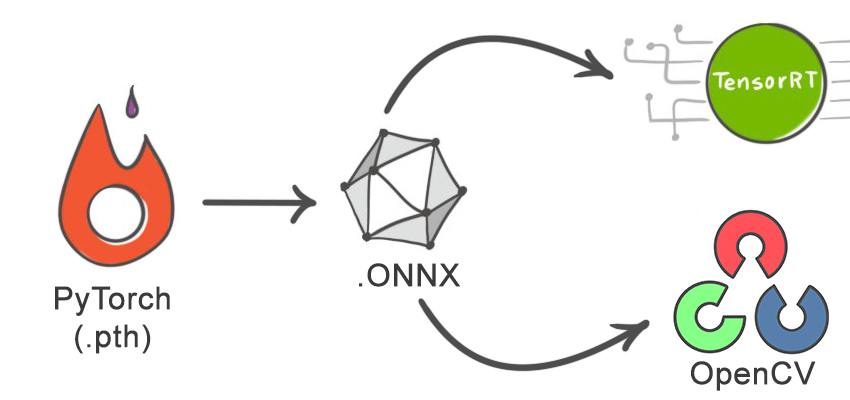
\includegraphics[width = \linewidth]{onnx convert.png}
    \centering
    \caption{Flusso di conversione di ogni modello.}
    \label{onnx-converter}
\end{figure}


\section{Supporto Cuda Frameworks}\label{acceleratori}
\subsection{TensorRT}
\begin{figure}
    \centering
    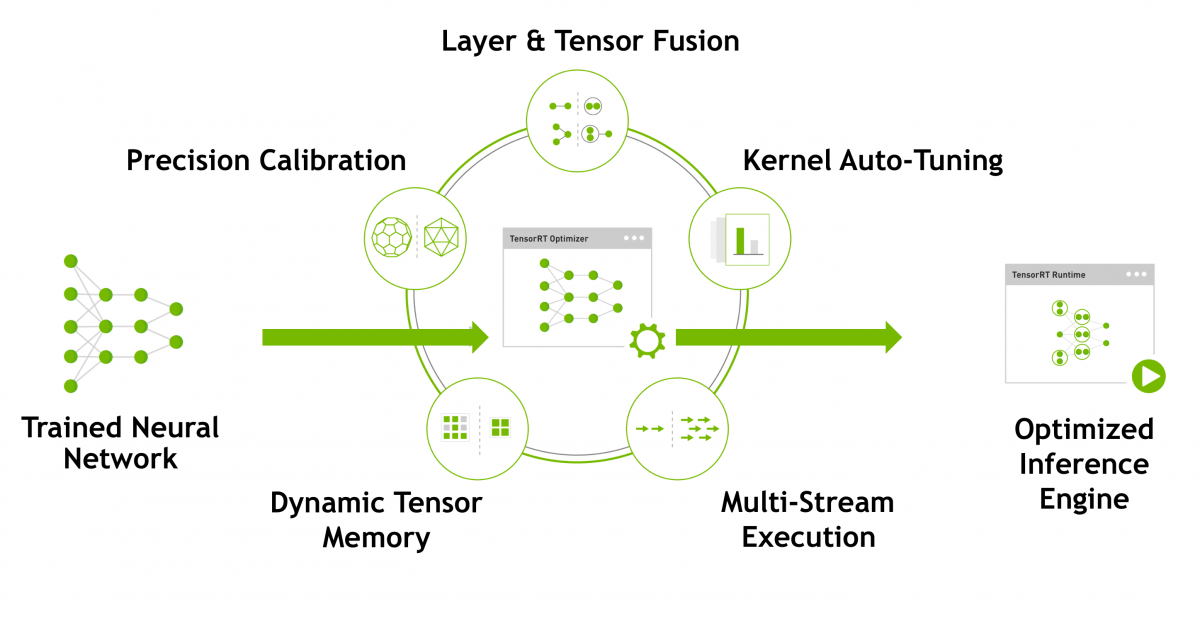
\includegraphics[width = \linewidth]{tensorrtOpt.png}
    \centering
    \caption{Ottimizzazioni si TensorRT sui modelli.}
    \label{tensorrt}
\end{figure}
TensorRT è un framework di machine learning, sviluppato interamente da 
NVidia, che esegue cinque diverse procedure di ottimizzazione su architetture 
basate su scheda GPU NVidia (Fig. (\ref{tensorrt})). 
\begin{enumerate}
    \item {\bfseries{\emph{Precision Calibration}}}: in questa ottimizzazione viene eseguita 
    l'operazione di \emph{Quantizzazione} che permette di mappare tutti i valori 
    dei pesi da una precisione FP32 bit a FP16 bit, creando una perdita 
    di precisione trascurabile.
    \item {\bfseries{\emph{Layer \& Tensor Fusion}}}: la seconda ottimizzazione riguarda l'eliminazione 
    di tutti quei layer che non vengono utilizzati, questo è 
    utile per poter evitare calcoli inutili. Successivamente, le operazioni 
    di Convoluzione, ReLU e normalizzazione Batch, vengono fuse in un 
    unico layer (\emph{CBR}). Questa operazione permette di eseguire calcoli 
    in una maniera più veloce ed efficace. Nella Figura (\ref{fusion_tensorrt}) si possono 
    vedere meglio quali sono tutti i layer che vengono fusi da TensorRT.
    \item {\bfseries{\emph{Kernel Auto-Tuning}}}: la terza ottimizzazione viene effettuata direttamente 
    sui filtri utilizzati nella rete. Durante questa fase vengono 
    selezionati i migliori layer, algoritmi e dimensioni di batch in base alla 
    piattaforma GPU di destinazione.
    \item {\bfseries{\emph{Dynamic Tensor Memory}}}: la gestione della memoria viene effettuata 
    proprio in questa ottimizzazione. TensorRT alloca memoria 
    solo per durante il periodo di vita di un tensore scongiurando un 
    sovraccarico di allocazioni permettendo esecuzioni rapide ed efficienti.
    \item {\bfseries{\emph{Multiple Stream Execution}}}: l'ultima ottimizzazione riguarda l'elaborazione 
    parallela di multipli flussi di input. Fondamentalmente, 
    questo è possibile utilizzando la libreria CUDA stream.
\end{enumerate}
L'aspetto più importante da ricordarsi, quando si utilizza TensorRT, è che 
bisogna assicurarsi che la procedura di ottimizzazione avvenga sulla stessa 
GPU NVidia che verrà utilizzata per l'inferenza. Questo deve avvenire 
in quanto TensorRT utilizza kernel specifici a seconda della piattaforma 
di destinazione. L'utilizzo di una ottimizzazione su una differente scheda 
grafica porta alla creazione di errori in fase di inferenza. 
\begin{figure}
    \centering
    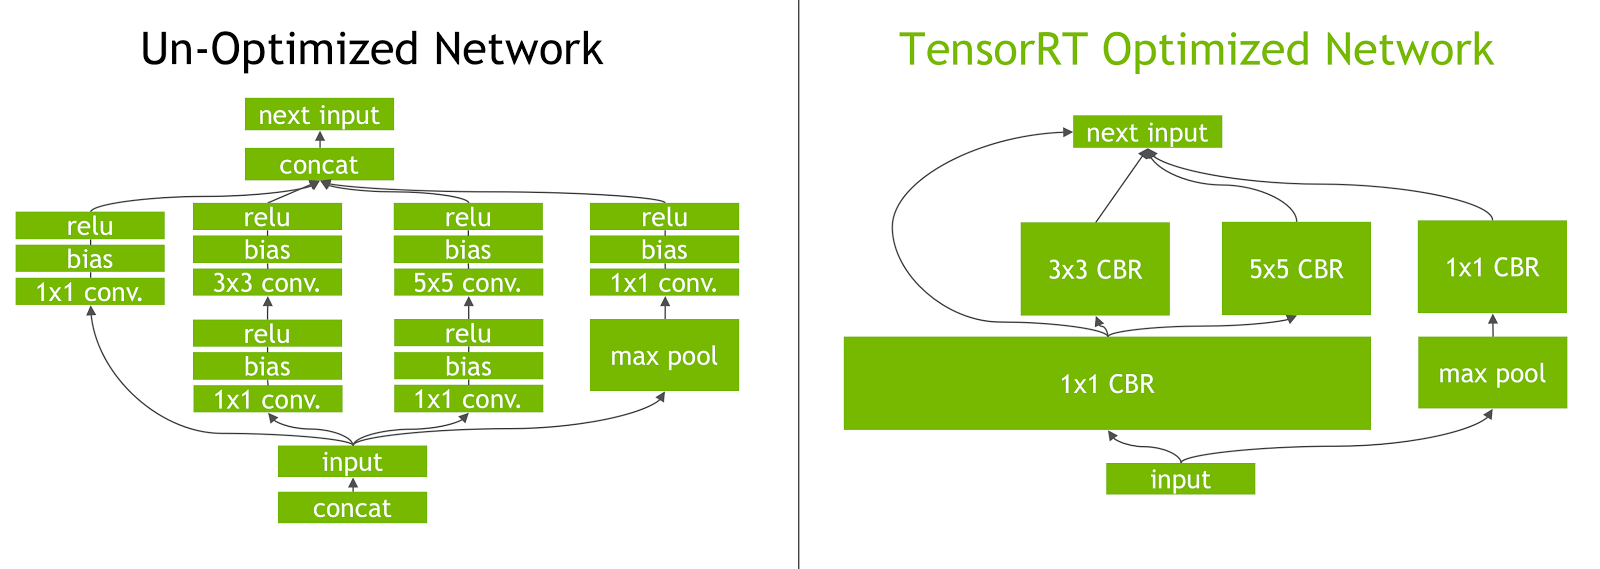
\includegraphics[width = \linewidth]{optTensor.png}
    \centering
    \caption{Fusione dei livelli Convolutional, Batch e ReLU eseguita da TensorRT.}
    \label{fusion_tensorrt}
\end{figure}

\subsection{NVidia Jetson utils}\label{utils}
NVidia dispone di una comunità che supporta l'evoluzione di tutte le sue schede 
embedded, inclusa la Jetson Nano. Questa associazione ha dato vita 
a delle librerie utilizzate in ambito di computer vision, nello specifico rivolto 
alla gestione e alla  progettazione di reti neurali. In ambito di inferenza, una 
parte di codeste utilizza l'acceleratore TensorRT per distribuire in modo 
efficiente le reti neurali sulla piattaforma Jetson utilizzata, consentendo 
un miglioramento delle prestazioni e al contempo una migliore efficienza 
energetica. Il codice sorgente messo a disposizione, sviluppato sia in linguaggio 
C++ che in Python (principalmente utilizzato in questo elaborato), 
è composto da diversi scripts che mirano ad eseguire i modelli per svolgere 
svariate attività:
\begin{itemize}
    \item \emph{ImageNet.py}: per attività di Image Recognition;
    \item \emph{DetectNet.py}: per attività di Object detection;
    \item \emph{SegNet.py}: per attività di Semantic Segmentation;
    \item \emph{PoseNet.py}: per attività di Pose Estimation.
\end{itemize}
Ognuno di questi ha lo scopo di eseguire l'inferenza di una apposita rete 
per produrre l'output inerente una specifica attività. In questa tesi sono 
stati utilizzati i primi tre scripts in quanto coerenti con lo scopo prefissato. 
L'input è costituito da uno stream di immagini, video o dati, proveniente 
da una sorgente esterna come per esempio una webcam esterna, collegata 
tramite una porta usb, oppure una webcam collegata tramite interfaccia 
CSI/ISP predisposta direttamente sulla scheda. I frame di input possono 
provenire da un file avente estensione jpeg, mp4, RTP, RTPS etc. Nel caso 
in cui l'input provenga da una fonte esterna, verrà utilizzato il protocollo 
V4L2 che imposterà il maggior numero di frame rate alla massima risoluzione 
supportata dalla fonte. Per quanto riguarda l'output, questo può 
essere distribuito nel medesimo formato di input. I codecs supportati dalla 
piattaforma sono i seguenti:
\begin{itemize}
    \item \emph{Decode}: H.264, H.265, VP8, VP9, MPEG-2, MPEG-4 e MJPEG;
    \item \emph{Encode}: H.264, H.265, VP8, VP9 e MJPEG.
\end{itemize}
Le APIs mettono a disposizione anche alcuni scripts che utilizzano il supporto 
CUDA in grado di gestire e manipolare le immagini, che siano di input o 
di output. Ritornando agli scripts principali, ImageNet accetta un'immagine 
in input e restituendone un intervallo di probabilità in output per ogni classe. 
DetectNet, a differenza di ImageNet, oltre a permette di concentrarsi sul rilevamento 
di oggetti, specifica la loro posizione tramite delle bounding boxes, 
all'interno del frame in input. Rispetto alla classificazione delle immagini, 
le reti utilizzate in questo contesto sono in grado di rilevare multipli oggetti, 
appartenenti alla stessa categoria e non, nell'input specificato. L'output 
prodotto è rappresentato da delle coordinate utili a delimitare i riquadri che 
contraddistinguono ogni singolo oggetto di ogni classe (Fig. \ref{detectnet_result}).
\begin{figure}
    \centering
    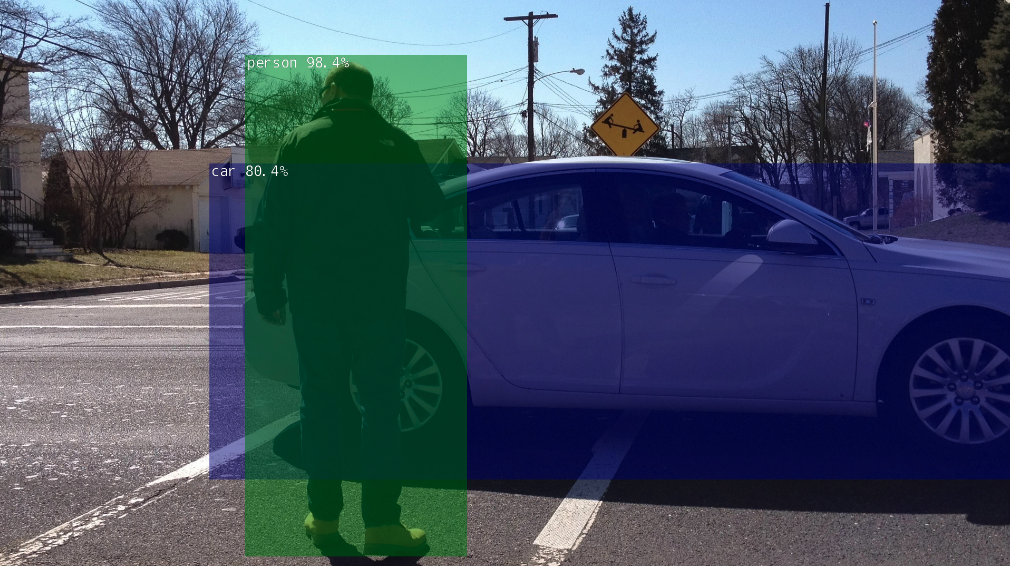
\includegraphics[width = \linewidth]{detectnet_result.png}
    \centering
    \caption{Esempio di ouput prodotto da DetectNet sulla Jetson Nano.}
    \label{detectnet_result}
\end{figure}
Per quanto 
riguarda l'attività di segmentazione semantica, questa viene interamente 
svolta dallo script Python Segnet. L'output prodotto da quest'ultimo si 
basa in un'immagine in cui vi è applicata una maschera sovrapposta utile a 
classificare ogni singolo pixel presente nell'immagine di input. Ogni pixel 
della maschera corrisponderà alla classe dell'oggetto sottostante classificato 
(Fig. \ref{segnet_result}).
\begin{figure}
    \centering
    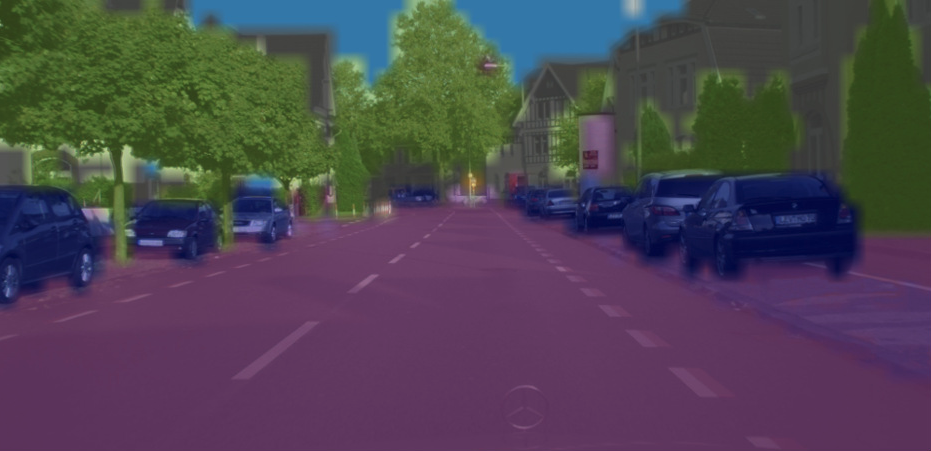
\includegraphics[width = \linewidth]{segnet_result.png}
    \centering
    \caption{Esempio di ouput prodotto da SegNet sulla Jetson Nano.}
    \label{segnet_result}
\end{figure}
Seppur non consigliata come piattaforma su cui effettuare il 
training di un modello, nella repository ufficiale \cite{repo_jetson_nano} viene riportato un link ad 
un'altra repository \cite{repo_pytorch_training} contenente il codice sorgente utile ad addestrare tutti 
i modelli impiegati nelle varie attività. Esiste una documentazione ufficiale 
contenente tutte le informazioni riguardanti gli script citati utilizzabili in 
ogni architettura presente nella famiglia Jetson \cite{Documentation_jetson}. Sia nel training che 
nell'inferenza di ogni modello, il framework di ML utilizzato è PyTorch.

\subsection{OpenCV}
Tra le tre architetture utilizzate in questo elaborato, una è sprovvista di una componente fondamentale utile ad accelerare l'allenamento e l'inferenza di un modello. I nuovi macbook pro, nonché il computer del sottoscritto, sono macchine che montano a bordo solo schede grafiche AMD. L'assenza di una scheda grafica NVidia implica l'utilizzo di librerie diverse da TensorRT il quale, a sua volta, fa uso delle librerie CUDA. Quando si verifica una tale limitazione, sia il training che l'inferenza vengono gestiti dalla componente principale di un computer: la CPU. Quando vi è un simile passaggio di elaborazione, le prestazioni computazionali sono nettamente inferiori rispetto a quelle ottenute su una scheda grafica. Ed eccoci giunti alla domanda principale: come può essere eseguito un modello su una piattaforma priva di una scheda grafica NVidia? A questo proposito ci viene in aiuto la nota libreria \emph{OpenCV}.
Principalmente utilizzata per lo sviluppo di applicazioni real-time rivolte alla visione artificiale e all'intelligenza artificiale. É in grado di fornire molteplici funzioni in grado di acquisire, analizzare e manipolare i dati visivi provenienti da uno specifica sorgete di input. Al suo interno, OpenCV possiede un modulo \emph{Deep Neural Network (DNN)} in grado di eseguire l'inferenza di un modello pre-addestrato direttamente su una CPU.
Questa libreria ha permesso di risolvere il problema inerente i test da svolgere sull'architettura Apple a disposizione. A partire dalla versione 4.2.0, OpenCV ha introdotto il pieno supporto alle schede grafiche GPU NVidia, sviluppando un nuovo modulo chiamato "\emph{cuDNN}".
Come ben si intuisce, gli autori hanno permesso di aumentare le performance utilizzando la capacità computazionale messa a disposizione di un hardware apposito. Tutto questo ha permesso di creare una sorta di accelerazione, lato inferenza, dei modelli pre-addestrati. Il supporto si è reso interessante per tutte quelle architetture che dispongono di una scheda grafica NVidia, prive di qualunque acceleratore come TensorRT. In questo elaborato, l'architettura che rientra in questa categoria è Google Colaboratory. A causa dell'impossibilità di installazione di TensorRT, si è preferito utilizzare il supporto messo a disposizione da OpenCV per poter ottenere i benchmarks voluti. Relativamente facile è risultata l'implementazione di questa funzionalità che ha permesso ad OpenCV di utilizzare la GPU messa a disposizione da Google. Le uniche due righe codice da poter aggiungere alla nostra rete (net) sono le seguenti:
\begin{itemize}
    \item \emph{net.setPreferableBackend(cv2.dnn.DNN\_BACKEND\_CUDA)}
    \item \emph{net.setPreferableTarget(cv2.dnn.DNN\_TARGET\_CUDA)}
\end{itemize}
Il resto del codice è uguale a quello utilizzato per l'inferenza su CPU.
Fondamentale risulta la conversione del modello pre-addestrato dal formato \emph{.pth} al formato \emph{.ONNX} per poter essere importato all'interno di OpenCV tramite la funzione \emph{readNetFromONNX()} messa sempre a disposizione nel modulo DNN.
Il supporto fornito da OpenCV ha permesso quindi di ottenere i benchmarks su entrambi le architetture utilizzate, ovvero sul macbook pro e su Google Colaboratory.

\section{Frames-per-Second (FPS)}
La velocità di inferenza rappresenta un indicatore di performance di ogni 
modello. Per poterla calcolare, la velocità di inferenza è rappresentata dai 
\emph{Frames-per-Second (FPS)} (\ref{FPS_Count}):
\begin{equation}\label{FPS_Count}
    FPS = \frac{1}{Ending \ Time - Starting \ Time}
\end{equation}
Questa misura è variabile e serve per rappresentare tre diversi elementi:
\begin{itemize}
    \item {\bfseries{\emph{Input}}}: ogni rete prende in input una sequenza di frame appartenenti 
    a un video/immagini. Ogni sequenza può avere un numero di FPS variabile. In 
    questo elaborato, vengono testati diversi video a 30FPS e a 60FPS.
    \item {\bfseries{\emph{Netwrok}}}: la velocità che la rete impiega ad effettuare uno specifico 
    task, può essere rappresentata dal numero di FPS. Riconoscere e/o 
    segmentare un oggetto appare essere un'attività onerosa in termini 
    computazionali, pertanto una rete è considerata veloce se, oltre a 
    produrre un output adeguato, svolge ogni task in un tempo breve.
    \item {\bfseries{\emph{Output}}}: il risultato prodotto da una rete è visibile solamente a 
    schermo. I video/immagini mostrati/e hanno una velocità di riproduzione 
    che è influenzata dal numero di FPS.
\end{itemize}
Tra le API messe a disposizione da NVidia, citate nella sezione \ref{utils}, 
fondamentale è risultato l'utilizzo dei metodi incaricati di calcolare la 
velocità d'inferenza, di input e di output raggiunta da ogni modello su ogni 
attività richiesta. 